\documentclass[11pt,a4paper]{article}
\usepackage[margin=2.4cm]{geometry}
\usepackage{lmodern}
\usepackage[T1]{fontenc}
\usepackage[utf8]{inputenc}
\usepackage{booktabs}
\usepackage{graphicx}
\usepackage{amsmath}
\usepackage{xcolor}
\usepackage{url}
\usepackage{tikz}
\usetikzlibrary{arrows.meta,calc,positioning}

\usepackage{fancyhdr}
\pagestyle{fancy}\fancyhf{}\renewcommand{\headrulewidth}{0pt}
\cfoot{\scriptsize Synthetic test material. All people, institutions, venues and results are fictional.}\rfoot{\small\thepage}
\fancypagestyle{plain}{\fancyhf{}\renewcommand{\headrulewidth}{0pt}\cfoot{\scriptsize Synthetic test material. All people, institutions, venues and results are fictional.}\rfoot{\small\thepage}}

\pdfinfoomitdate=1
\pdftrailerid{}
\pdfsuppressptexinfo=-1
\pdfinfo{/Title (Quillwave: Sparse-Sensor Reconstruction of Synthetic Ripple Fields) /Author (Ada Placeholder; Ben Example; Cleo Sample) /Subject (FICTIONAL synthetic test material) /Keywords (fictional; synthetic; test fixture; CC0 1.0; paper) /Creator (Quillwave kit generator)}

\graphicspath{{../../figures/}}
\begin{document}
\begin{center}
{\LARGE\bfseries Quillwave: Sparse-Sensor Reconstruction of Synthetic Ripple Fields\par}\vspace{10pt}
{\large Ada Placeholder$^{1}$ \quad Ben Example$^{1}$ \quad Cleo Sample$^{1}$\par}\vspace{4pt}
{\small $^{1}$Example University (fictional), Department of Imaginary Sciences\par}\vspace{2pt}{\small \texttt{ada@example.invalid}, \texttt{ben@example.invalid}, \texttt{cleo@example.invalid}\par}
\vspace{4pt}{\small Accepted at FCSV 2026 (Fictional Conference on Synthetic Vision).\par}
\end{center}
\begin{abstract}
Quillwave reconstructs a full $256\times256$ ripple field from 64 point sensors. Ripple
fields are procedurally generated sums of interfering circular waves: cheap to synthesise, but hard to
interpolate, because the wave fronts between sensors are lost by smooth interpolation. Quillwave encodes the
sensor readings into a 128-dimensional latent field code and decodes it with a coordinate-based field
decoder. On RippleBench-Synthetic, a benchmark of 500 synthetic test fields generated for this work,
Quillwave reaches 29.46\,dB PSNR and 0.887 SSIM, 5.41\,dB above radial-basis interpolation (the
best baseline), which is a 71.2\,\% lower mean squared error. It is also 1.36$\times$ faster than
radial-basis interpolation at inference. All results are on synthetic fields only.
\end{abstract}

\section{Introduction}
Many sensing problems share one shape: a handful of point measurements, and a wish to know the
whole field between them. Smooth interpolation is the standard answer, and it works when the field is
smooth. It fails for fields made of travelling waves, where the interesting structure, the wave fronts,
lies exactly between the sensors.

We study this failure on \emph{ripple fields}: sums of damped circular waves from a few random sources,
sampled on a $256\times256$ grid. They are easy to generate in any quantity, have a known ground truth,
and carry no personal or proprietary data. We make three contributions:
\begin{itemize}
\item RippleBench-Synthetic, a procedurally generated benchmark with 2000 training and 500 test fields;
\item Quillwave, an encoder--decoder that predicts the full field from 64 sensors and a per-pixel confidence;
\item an evaluation against linear and radial-basis interpolation and an ablation, Quillwave-Lite.
\end{itemize}

\section{Related work}
Interpolating sparse probes of wave-like fields has been studied with hand-crafted
bases~\cite{nobody2024interpolating,anyone2023radial} and, more recently, with learned
decoders~\cite{someone2025learned}. Sensor placement in toy domains is discussed
in~\cite{whoever2024placement}; we fix the layout to isolate the reconstruction step. Purely synthetic
benchmarks~\cite{nameless2025benchmarks} trade realism for control, and we follow the error measures
recommended in~\cite{anybody2025measuring}.

\section{Method}
\begin{figure}[t]\centering
\resizebox{\linewidth}{!}{% Quillwave overview diagram (FICTIONAL synthetic test material). Same file is used
% for figures/overview.png (standalone) and inside the paper.
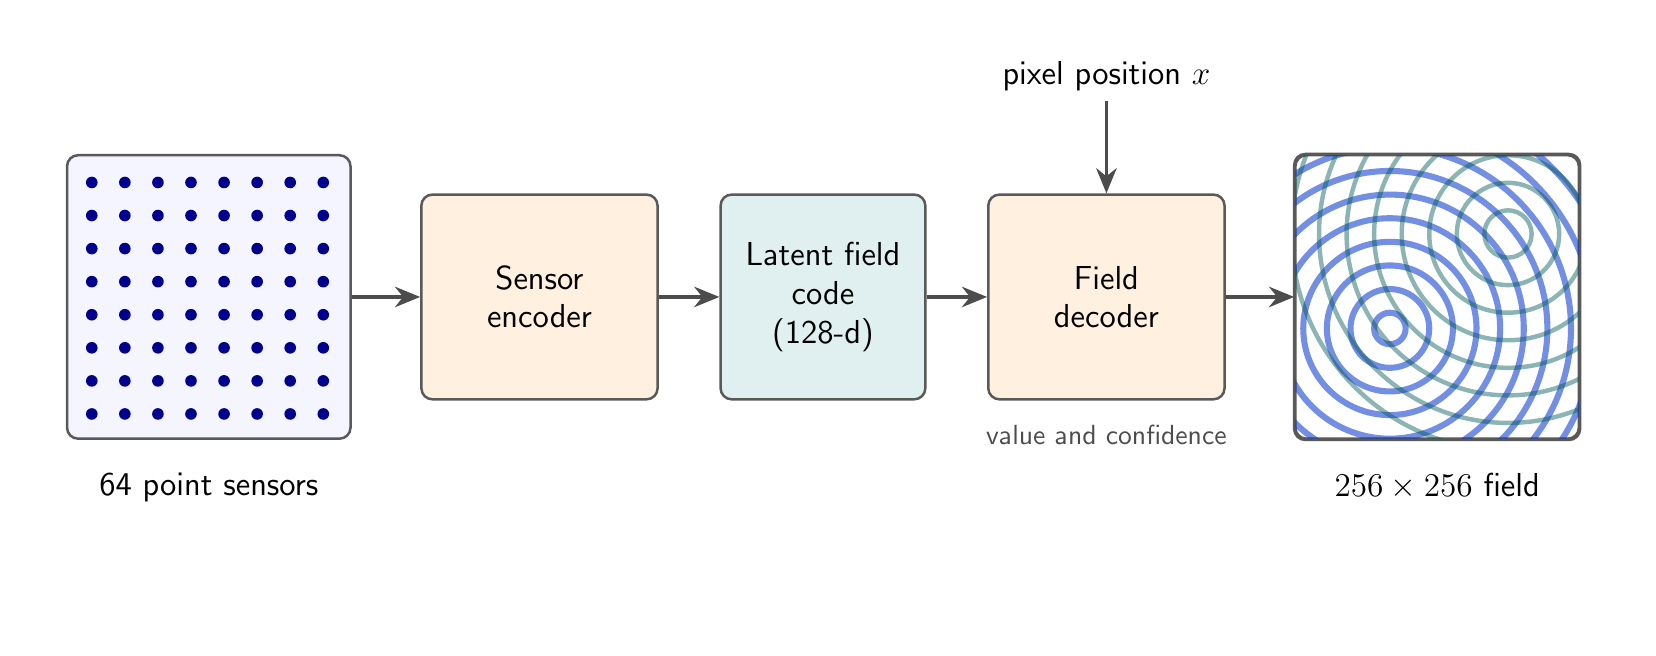
\begin{tikzpicture}[x=1cm,y=1cm,font=\sffamily,
  box/.style={draw=black!65, line width=0.9pt, rounded corners=4pt, align=center,
              minimum height=2.6cm, minimum width=3.0cm, font=\sffamily\large},
  arr/.style={-{Stealth[length=3.2mm,width=2.6mm]}, line width=1.2pt, black!70}]
\useasboundingbox (0,0) rectangle (20.32,7.62);
% sensors
\node[box, fill=blue!4, minimum width=3.6cm, minimum height=3.6cm] (s) at (2.3,4.2) {};
\foreach \i in {0,...,7}{\foreach \j in {0,...,7}{
  \fill[blue!55!black] ($(s.south west)+({0.33+\i*0.42}, {0.33+\j*0.42})$) circle (2.1pt);}}
\node[font=\sffamily\large, below=3mm of s] {64 point sensors};
% encoder, latent, decoder
\node[box, fill=orange!12] (e) at (6.5,4.2) {Sensor\\encoder};
\node[box, fill=teal!12, minimum width=2.6cm] (z) at (10.1,4.2) {Latent field\\code\\(128-d)};
\node[box, fill=orange!12] (d) at (13.7,4.2) {Field\\decoder};
% output field: concentric ripples clipped to a square
\node[box, fill=white, minimum width=3.6cm, minimum height=3.6cm] (o) at (17.9,4.2) {};
\begin{scope}
\clip[rounded corners=4pt] (o.south west) rectangle (o.north east);
\foreach \r in {0.2,0.5,...,3.2}{\draw[blue!60!teal, line width=2.2pt, opacity=0.55] ($(o.center)+(-0.6,-0.4)$) circle (\r);}
\foreach \r in {0.3,0.65,...,3.0}{\draw[teal!70!black, line width=1.6pt, opacity=0.45] ($(o.center)+(0.9,0.8)$) circle (\r);}
\end{scope}
\draw[black!65, line width=0.9pt, rounded corners=4pt] (o.south west) rectangle (o.north east);
\node[font=\sffamily\large, below=3mm of o] {$256\times256$ field};
% query coordinate
\node[font=\sffamily\large] (q) at (13.7,7.0) {pixel position $x$};
\draw[arr] (q) -- (d);
\node[font=\sffamily, text=black!70] at (13.7,2.45) {value and confidence};
\draw[arr] (s) -- (e); \draw[arr] (e) -- (z); \draw[arr] (z) -- (d); \draw[arr] (d) -- (o);
\end{tikzpicture}
}
\caption{Quillwave pipeline: sensor readings are encoded into a latent field code, which a coordinate-based
decoder turns into the full field.}\label{fig:overview}
\end{figure}

Let $s\in\mathbf{R}^{64}$ be the sensor readings at known positions $p_i$ on a regular
$8\times8$ grid. The sensor encoder $E_\phi$ maps the pairs $(p_i, s_i)$ to a latent field code
$z = E_\phi(s) \in \mathbf{R}^{128}$. The field decoder $D_\theta$ is coordinate-based: for any pixel
position $x$ it predicts a value and a confidence,
\begin{equation}
  \bigl(\hat f(x),\, c(x)\bigr) = D_\theta(x, z).
\end{equation}
Training minimises the mean squared error between $\hat f$ and the ground-truth field over all pixels,
plus a term that asks $c(x)$ to rank pixels by their error. Quillwave-Lite removes the latent code and
conditions the decoder on the raw readings directly. The full model has 1.2M parameters and is trained
for 200 epochs.
\paragraph{Encoder.} Each sensor contributes a token made of its position and its reading. The tokens
pass through a small set-encoder with shared weights followed by attention pooling, so the code does not
depend on the order in which sensors are listed. The pooled vector is projected to the latent field code.

\paragraph{Decoder.} The decoder receives a pixel position, encoded with sinusoidal features, together
with the latent field code. A stack of fully connected layers with skip connections predicts two outputs:
the field value and a confidence score. Because the decoder is queried per pixel, the output resolution is
not tied to the training resolution, although every result in this document uses the benchmark resolution.

\paragraph{Confidence.} The confidence head is trained with a ranking objective: pixels with a larger
reconstruction error should receive a lower score. It is meant to show \emph{where} the reconstruction is
least reliable, not \emph{how} reliable it is; Section~\ref{sec:limits} returns to this point.

\section{Experiments}
\subsection{Setup}
RippleBench-Synthetic fields are $256\times256$ sums of damped circular waves from up to four
sources with random positions, wavelengths and phases. We use 2000 training fields and 500 test fields,
and 64 sensors unless stated otherwise. We compare against linear interpolation and radial-basis
interpolation from the same sensors, and against the Quillwave-Lite ablation. Learned models are trained
5 times with different seeds; we report the mean over the 5 training runs. Runtime is per
field at inference.
\begin{table}[t]\centering\small
\caption{Reconstruction quality on RippleBench-Synthetic (64 sensors, $256\times256$ fields, mean over 5 training runs). Higher PSNR/SSIM is better; lower runtime is better.}\label{tab:main}
\begin{tabular}{lrrr}\toprule
Method & PSNR (dB) $\uparrow$ & SSIM $\uparrow$ & Runtime (ms) $\downarrow$ \\\midrule
Linear interpolation & 21.37 & 0.612 & \textbf{0.8} \\
Radial-basis interpolation & 24.05 & 0.701 & 6.4 \\
Quillwave-Lite (ablation) & 27.82 & 0.834 & 3.1 \\
Quillwave (ours) & \textbf{29.46} & \textbf{0.887} & 4.7 \\
\bottomrule\end{tabular}
\end{table}

\begin{table}[t]\centering\small
\caption{PSNR (dB) on RippleBench-Synthetic as the number of sensors changes ($256\times256$ fields).}\label{tab:sweep}
\begin{tabular}{lrrrr}\toprule
Method & 16 sensors & 32 sensors & 64 sensors & 128 sensors \\\midrule
Linear interpolation & 16.92 & 19.10 & 21.37 & 23.88 \\
Radial-basis interpolation & 18.44 & 21.26 & 24.05 & 26.71 \\
Quillwave-Lite (ablation) & 21.03 & 24.67 & 27.82 & 30.15 \\
Quillwave (ours) & \textbf{22.58} & \textbf{26.31} & \textbf{29.46} & \textbf{31.94} \\
\bottomrule\end{tabular}
\end{table}

\subsection{Results}
Table~\ref{tab:main} gives the main result. Quillwave reaches 29.46\,dB PSNR and 0.887 SSIM,
5.41\,dB above radial-basis interpolation, the best baseline; in terms of mean squared error this is a
71.2\,\% reduction. At 4.7\,ms per field it is 1.36$\times$ faster than radial-basis interpolation
(6.4\,ms), though slower than linear interpolation (0.8\,ms). The ablation Quillwave-Lite reaches
27.82\,dB, so the latent field code accounts for part of the gain.

Table~\ref{tab:sweep} varies the number of sensors. Quillwave is the best method at every sensor count,
from 22.58\,dB with 16 sensors to 31.94\,dB with 128 sensors. Figure~\ref{fig:panels}
summarises these trends together with error statistics and the training curve, and
Figure~\ref{fig:qual} shows reconstructions of four test scenes.
\begin{figure}[t]\centering
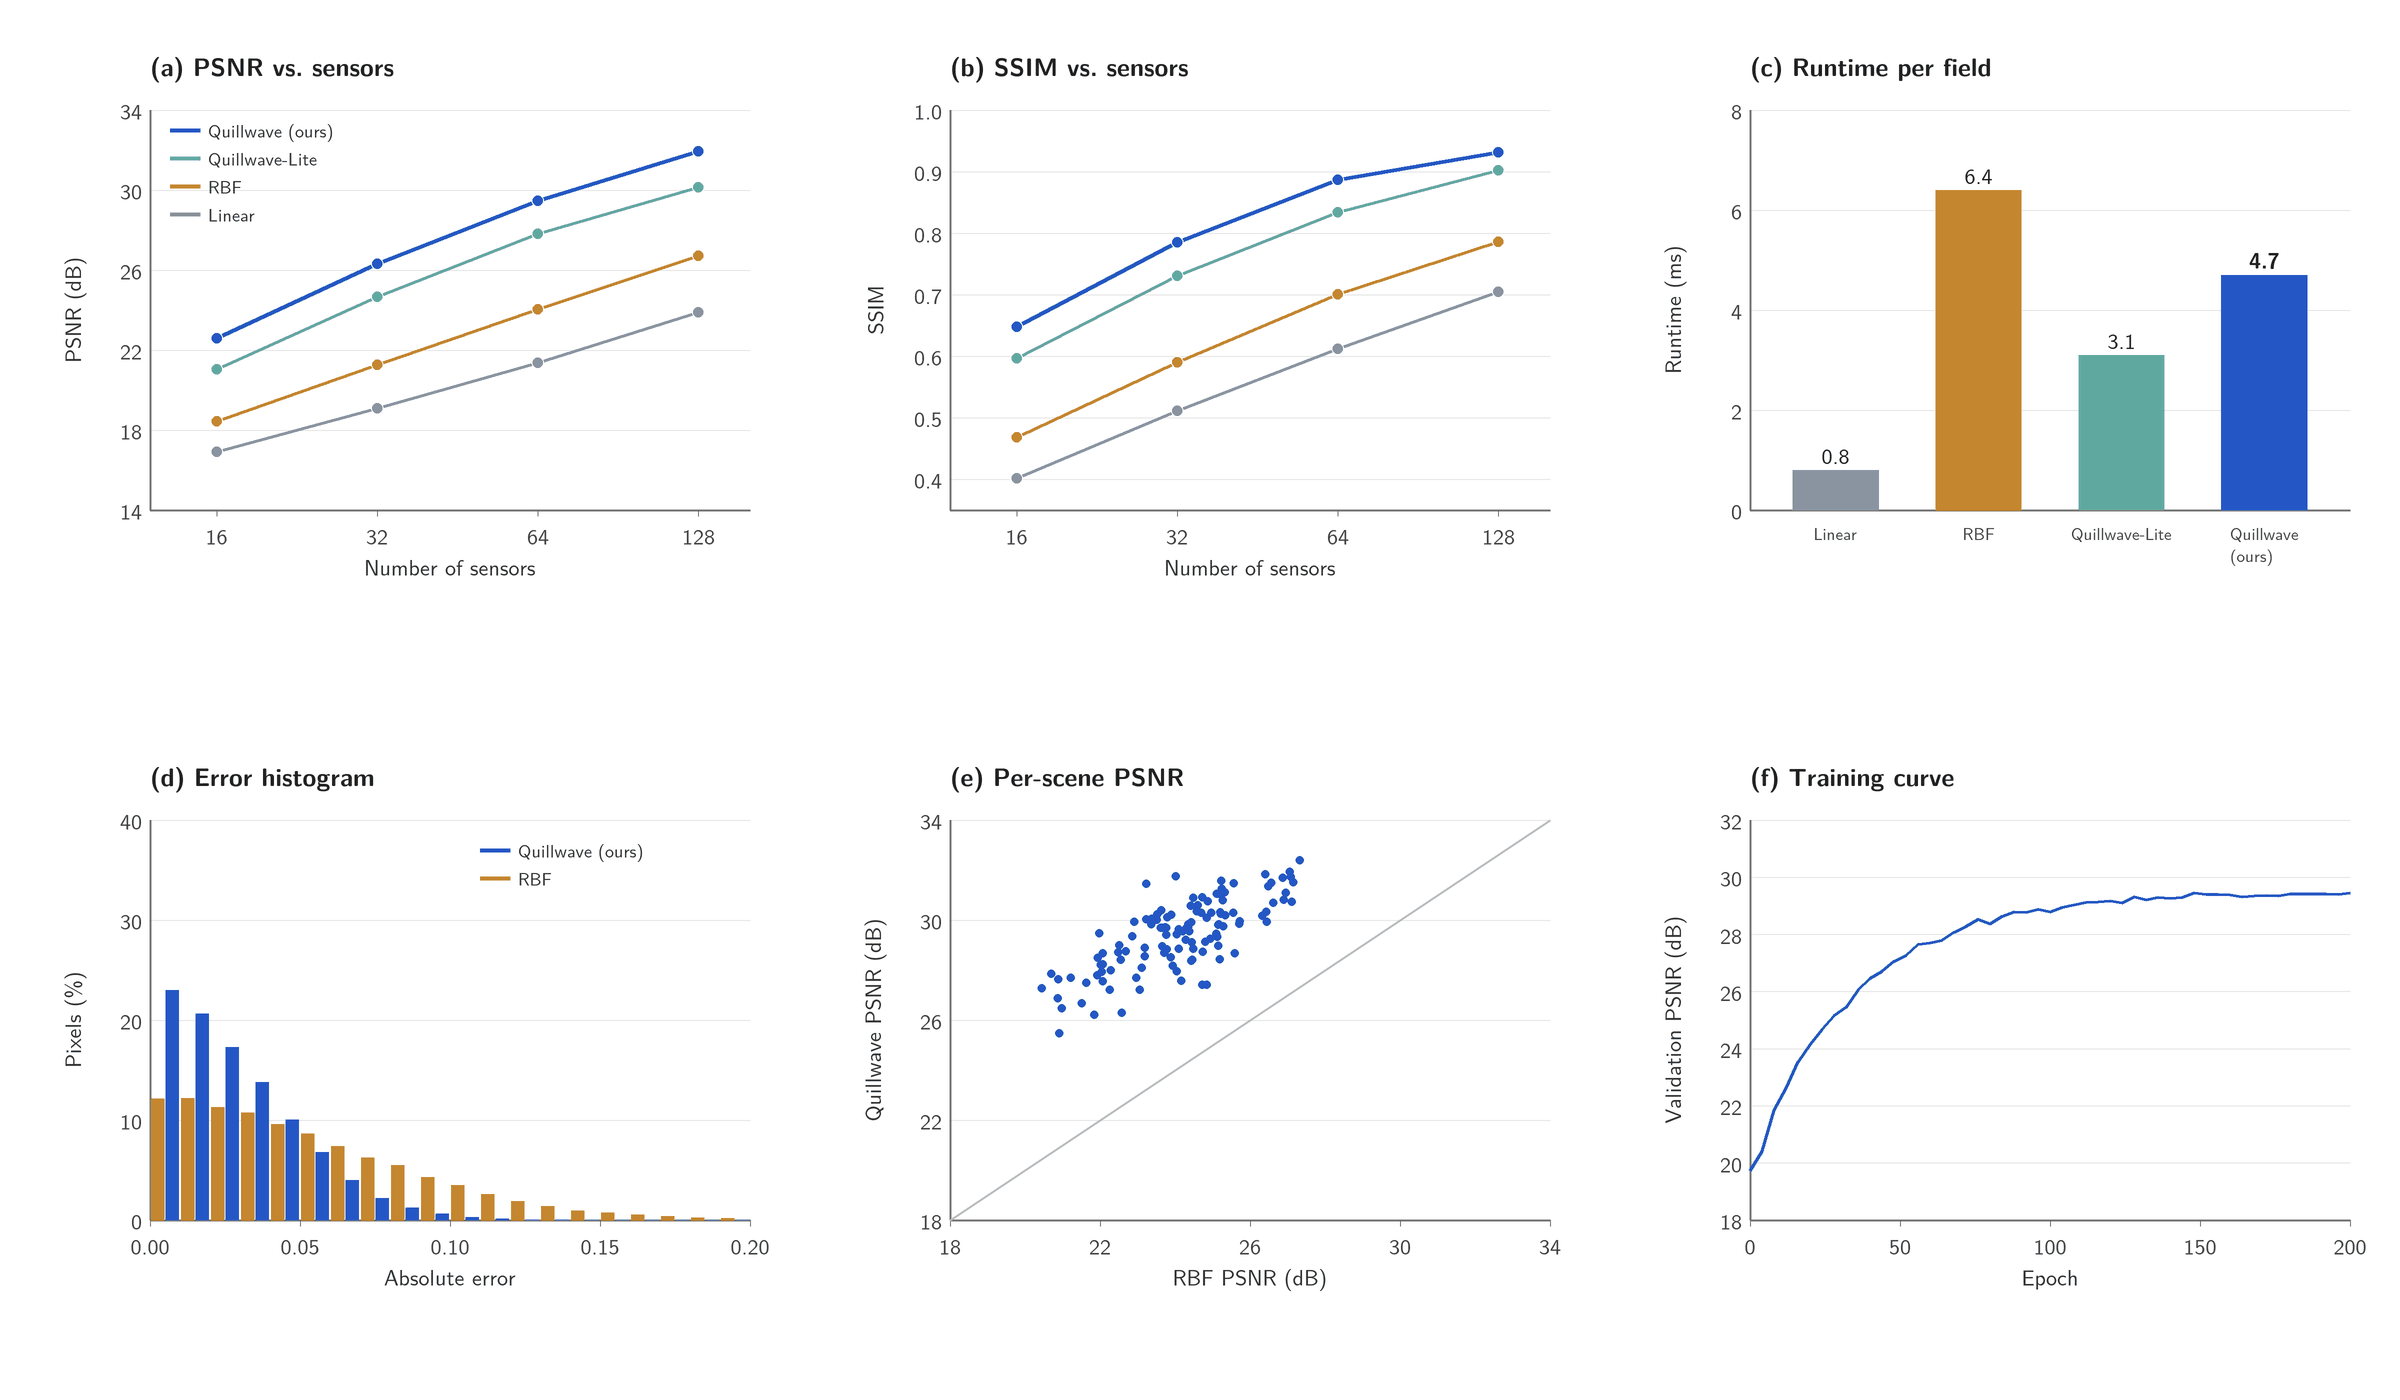
\includegraphics[width=\linewidth]{results_panels.png}
\caption{Results on RippleBench-Synthetic. (a) PSNR and (b) SSIM against the number of sensors; (c) runtime;
(d) absolute error histogram; (e) per-scene PSNR, Quillwave against radial-basis interpolation;
(f) validation PSNR during training.}\label{fig:panels}
\end{figure}

\begin{figure}[t]\centering
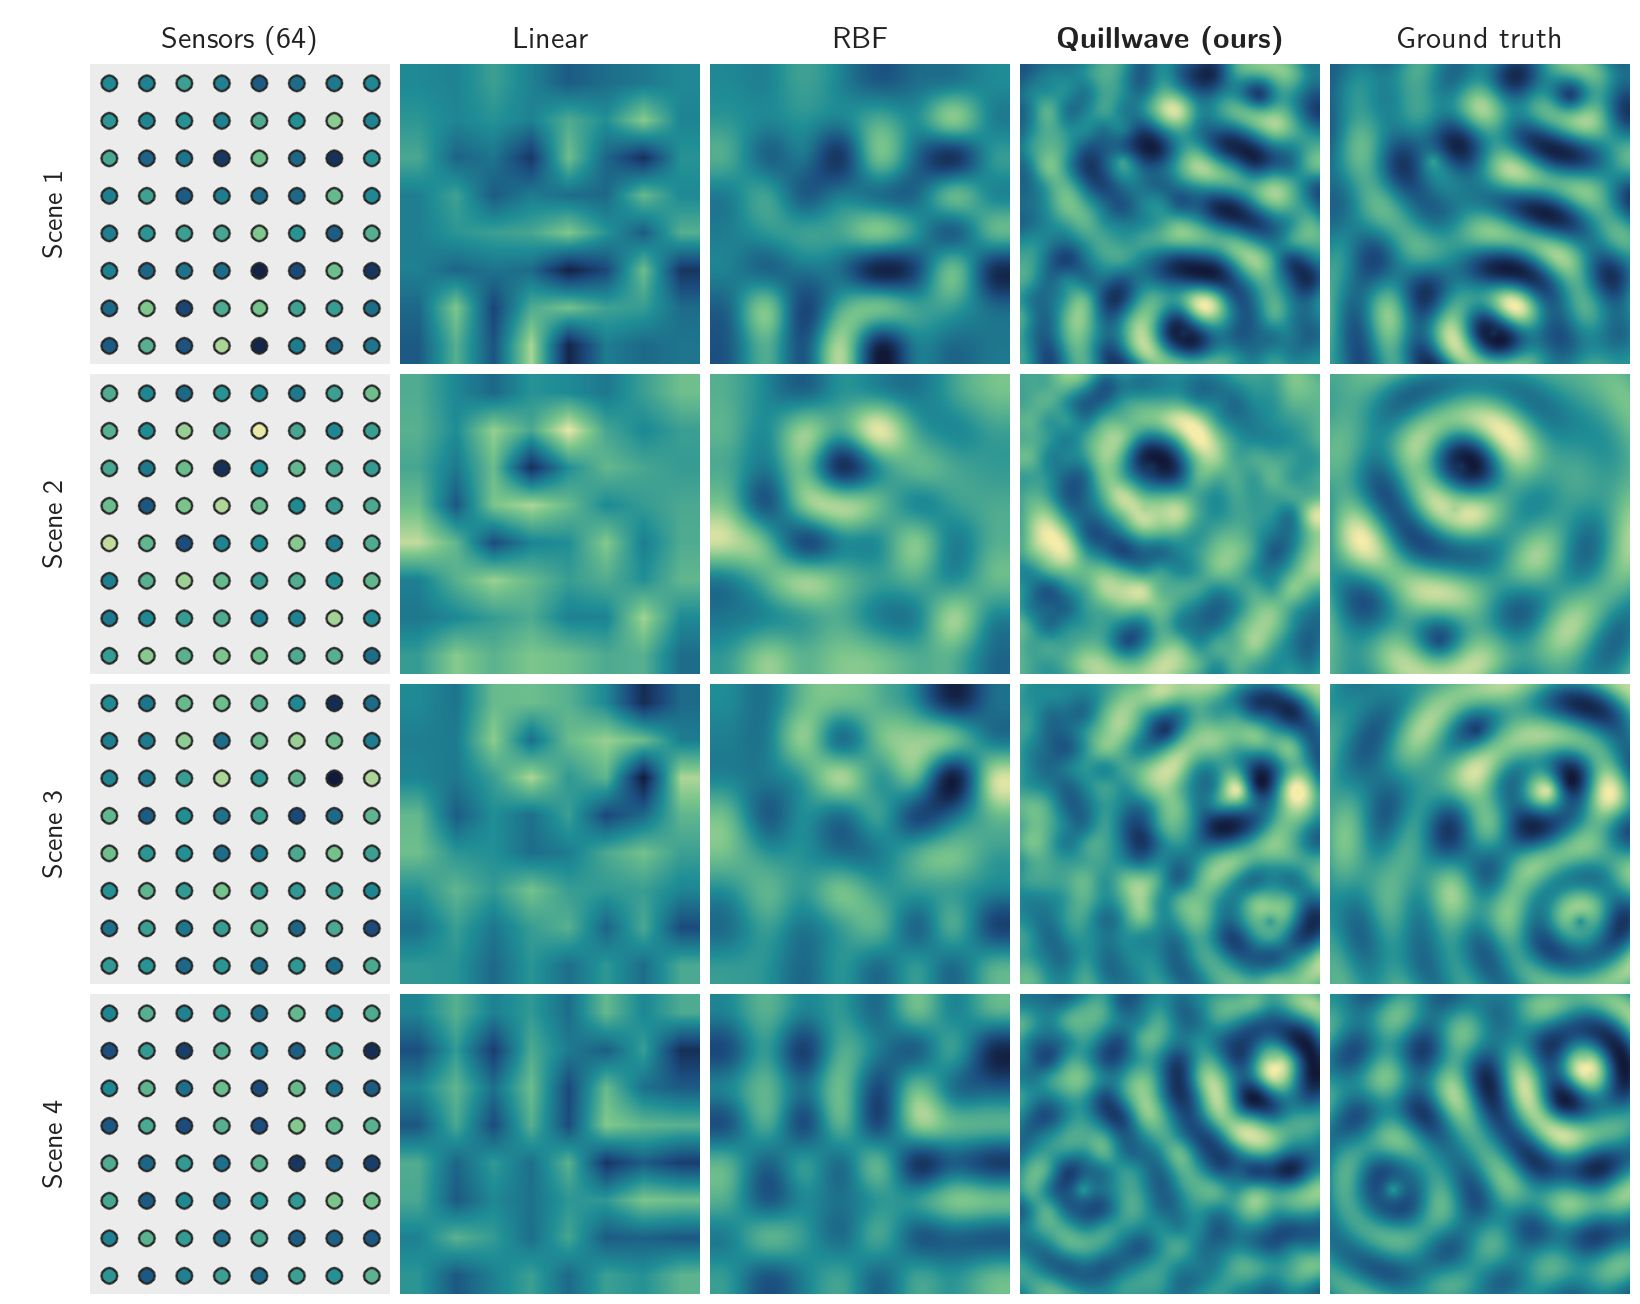
\includegraphics[width=\linewidth]{qualitative_grid.jpg}
\caption{Four test scenes: sensor map, linear interpolation, radial-basis interpolation, Quillwave, and
ground truth.}\label{fig:qual}
\end{figure}

\paragraph{Failure cases.} Quillwave is least accurate where two wave sources lie close together
between the same group of sensors: the interference pattern then varies faster than the sensor spacing,
and the decoder tends to merge the two sources into one. Radial-basis interpolation fails in the same
places, but more smoothly. Near the border of the field, where sensors are present only on one side, all
methods lose accuracy; Quillwave keeps the wave fronts but sometimes shifts their phase.
\subsection{User study}
A small user study with 20 participants rated the side-by-side comparison videos. Mean
ease of use was 4.10 and mean perceived quality 3.90 on a scale up to 5. Raw responses are not
published.

\section{Discussion}
The results suggest that the main benefit of a learned latent code is a prior over plausible wave
patterns: with few sensors, the decoder fills the gaps with wave fronts that are consistent with the
readings, where interpolation fills them with a smooth surface. This prior is also the main risk. Because
RippleBench-Synthetic is generated by the same family of processes used for training, the benchmark
rewards exactly this prior, and it says little about fields from other processes. A fair comparison on
real measurements would need baselines with access to the same training data and the same compute budget,
and a separate check of whether the confidence scores match observed errors.

\section{Limitations}\label{sec:limits}
\begin{itemize}
\item \textbf{Baselines are not compute-matched.} Quillwave is trained for 3.5 GPU-hours, while the interpolation baselines need no training at all.
\item \textbf{Synthetic fields only.} Every result is on RippleBench-Synthetic; no real sensor data was used, and behaviour on real measurements is unknown.
\item \textbf{Confidence is not calibration.} The per-pixel confidence map that Quillwave outputs has not been checked against observed error rates, so it should not be read as a calibrated probability.
\end{itemize}


\section{Conclusion}
Quillwave shows that a learned latent field code recovers wave fronts that smooth interpolation
misses, at a lower runtime than radial-basis interpolation. Whether this carries over to real
measurements is open; the limitations above apply to every number in this document.

\begin{thebibliography}{9}\small
\bibitem{nobody2024interpolating} Q. Nobody and R. Anyone. Interpolating ripples from very few probes. \emph{Proc. FCSV 2024}, 2024. (Fictional reference.)
\bibitem{anyone2023radial} R. Anyone. Radial bases for sparse synthetic fields. \emph{J. Imaginary Sci.}, 2023. (Fictional reference.)
\bibitem{someone2025learned} S. Someone and Q. Nobody. Learned decoders for synthetic wave fields. \emph{Proc. FCSV 2025}, 2025. (Fictional reference.)
\bibitem{whoever2024placement} T. Whoever. A note on sensor placement in toy domains. \emph{J. Imaginary Sci.}, 2024. (Fictional reference.)
\bibitem{nameless2025benchmarks} U. Nameless and S. Someone. Benchmarks without data. \emph{Proc. FCSV 2025}, 2025. (Fictional reference.)
\bibitem{anybody2025measuring} V. Anybody. On measuring reconstruction error. \emph{J. Imaginary Sci.}, 2025. (Fictional reference.)
\end{thebibliography}

\end{document}
